\section{Modélisation des pangénomes et premières observations}
\label{sec:pan_model}

Pour développer des méthodes d'analyse et de construction de pangénome, il faut tout d'abord définir le modèle pangénomique. La modélisation va principalement répondre à 3 questions : 
\begin{itemize}
    \item de quoi est composé le pangénome et comment classer ses composants ?
    \item comment représenter le pangénome, quelle structure mathématique utiliser ? 
    \item comment le pangénome évolue lorsque l'on ajoute des séquences ? 
\end{itemize}

Je répondrai à ces questions en présentant les modèles les plus répandues et qui permettront de présenter les méthodes de construction et d'analyse de pangénome les plus utilisées. 

\subsection{Les différents types de pangénomes}

Les pangénomes peuvent être divisés en 2 catégories en fonction de l'unité choisit pour les construire. Le premier type, celui présenté par Tettelin \textit{et al.} \cite{tettelin_genome_2005}, utilise les gènes comme unité de base du pangénome (\autoref{fig:panType}.B). En regroupant les gènes par homologie (appelé famille de gènes, cf. \autoref{sec:fam}), il est possible d'obtenir la présence/absence de gènes similaire dans les génomes. Ces pangénomes ont l'avantage d'être moins couteux en ressources de calcul pour être construit. De plus, ils sont faciles à interpréter, car les gènes sont des unités déjà bien définies et parfois, ils sont même annotés fonctionnellement. Néanmoins, en utilisant les gènes, la méthode d'annotation à un impact important sur le pangénome et il est sensible aux erreurs d'annotation. De plus, les régions non codantes ne sont pas prises en compte dans cette approche. Enfin, les SNPs peuvent passer inaperçu après le regroupement, ainsi que les variants structuraux (SV).

L'autre type de pangénome est basé sur les séquences brutes des génomes. Cette approche plus récente, qui peut être associé à l'outil GenomeMapper \cite{schneeberger_simultaneous_2009}, permet d'identifier les parties similaires des parties variables à partir d'un alignement complet des séquences (\autoref{fig:panType}.C,D). Cette approche a l'intérêt de prendre en compte toute la diversité des génomes (codant, non codant, SNPs et SV). Toutefois, la construction de ces pangénomes est plus coûteuse en ressources. De plus, l'interprétation est plus complexe, car le pangénome n'est pas annoté au départ. Pour terminer, certaines méthodes de construction, utilise un génome de référence comme séquence de base (\autoref{fig:panType}.C), ce qui peut aussi introduire un biais.
    

\begin{figure}[htbp]
    \centering
    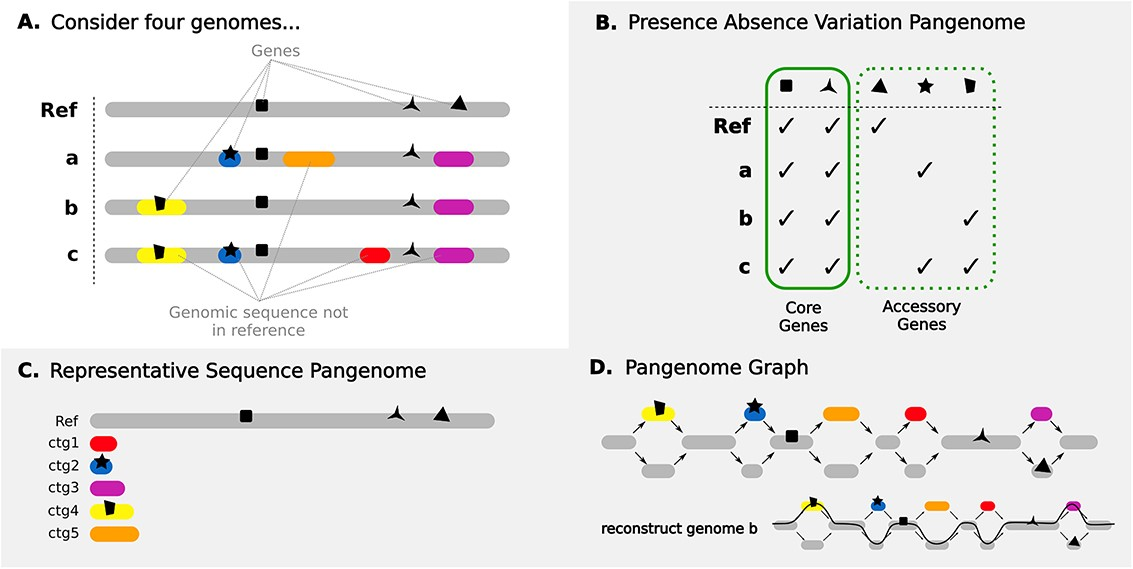
\includegraphics[width=0.8\linewidth]{images/pangenomeTypes.jpeg}
    \caption[Différents types de pangénomes]{Différents types de pangénomes. Extrait de \cite{matthews_gentle_2024}}
    \label{fig:panType}
\end{figure}

\subsection{Pangénome basé sur les gènes}

\subsubsection{Partitionnement des familles de gènes}

Une fois que les génomes ont été annotés et les familles de gènes construites, cette approche pangénomique permet de classer les gènes en fonction de la présence/absence de leur famille dans les génomes. Les familles vont être séparées en 2 parties (\autoref{fig:pangenome2}), les familles qui sont présentes dans tous les génomes sont dites "c\oe ur" (\textit{core} en anglais) et les autres sont dites "accessoire" (\textit{accessory} ou \textit{dispensable} en anglais). Cette dichotomie en \textit{core genome} et \textit{accessory genome} est liée au caractère essentiel ou non des fonctions codées par les gènes. Les familles "\textit{core}" sont impliquées dans les processus cellulaires vitaux, ce qui crée une forte pression de sélection de leurs gènes et une forte conservation dans l'ensemble des génomes. À l'inverse, les familles accessoires sont plutôt liées à des adaptations à l'environnement, un mode de vie\dots. Leurs gènes sont donc moins soumis à la pression de sélection et donc moins conservé dans les génomes.

\begin{figure}[htbp]
    \centering
    \subfloat[Pangénome bipartie]{
        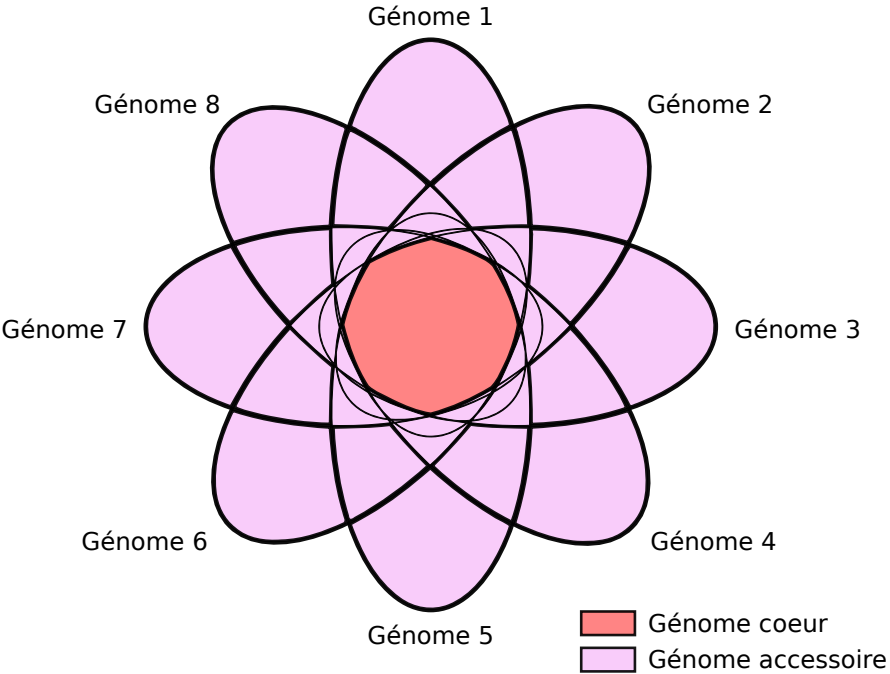
\includegraphics[width=0.48\linewidth]{images/pangenome2.png}
        \label{fig:pangenome2}
    }
    \hfill
    \subfloat[Pangénome tripartie]{
        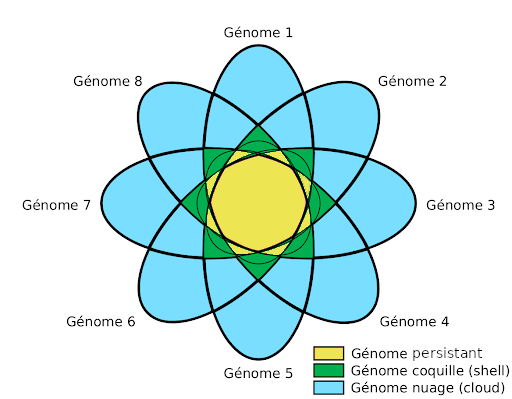
\includegraphics[width=0.48\linewidth]{images/pangenome3.png}
        \label{fig:pangenome3}
    }
    \caption[Partitionnement des pangénomes.]{Partitionnement des pangénomes. Extrait et adapté de \cite{gautreau_conceptualisation_2020}}
    \label{fig:pangenomeVenn}
\end{figure}

Ce partitionnement du pangénome en 2 parties, bien que largement utilisé, est une vision très stricte de la distribution des gènes dans les génomes, qui peut amener à des erreurs d'interprétation. Il faut d'abord prendre en compte que même si le nombre de génomes disponible est de plus en plus conséquent, il n'est toutefois pas possible d'avoir l'ensemble des génomes d'une espèce (cf. \autoref{sec:croissance_pan}), ce qui implique qu'il est plus que probable que des gènes soient placés dans l'accessoire alors qu'ils sont \textit{core} et inversement. De plus, les techniques de séquençage et les outils bioinformatique ne sont pas infaillibles, et donc une erreur d'assemblage, d'annotation, de regroupement en famille, ou encore l'utilisation de génome partiel, peut entraîner le mauvais classement d'une famille. Pour répondre à ce problème, Lapierre et Gogarten \cite{lapierre_estimating_2009} suggère de définir un c\oe ur relaché (\textit{soft-core} en anglais), qui contient les familles présente dans 95 \% des génomes\footnote{pourcentage peut varier en fonction des études.}. Une autre proposition, de Snippen \textit{et al.} \cite{snipen_microbial_2009} raffinant un modèle proposé par Hogg \textit{et al.} \cite{hogg_characterization_2007}, rendrait le nombre de partitions variable en fonction du contenu du pangénome. Cette dernière proposition, permet de ne pas utiliser de seuil fixe pour partitionner les familles. En parallèle, Koonin \textit{et al.}, dans une analyse de l'ensemble des génomes procaryotes disponible en 2008 \cite{koonin_genomics_2008}, et Makarova \textit{et al.}, en étudiant l'ensemble des génomes archées disponible en 2007 \cite{makarova_clusters_2007}, propose une vision du pangénome en tripartie (\autoref{fig:pangenome3}). Dans les 2 articles, les génomes sont annotés fonctionnellement, puis, pour chaque annotation, on représente le nombre de génomes la présentant. Dans les 2 cas, ils obtiennent une courbe en U, dont chaque côté représente une partie et la base une autre partie. Ils redéfinissent alors le \textit{core genome} comme les gènes conservés ou quasiment dans tous les génomes. Ce \textit{core genome} relâché et flexible (sans seuil) est aussi appelé \textit{persistent genome} dans certains articles pour le différencier du \textit{core genome} définit en premier. L'\textit{accessory genome} sera lui diviser en 2, le \textit{cloud genome} correspondant aux gènes partagé par un faible nombre de génomes, et le \textit{shell genome} correspondant aux gènes ayant une fréquence intermédiaire dans les génomes. Ces différents partitionnements, qui ne sont pas incompatibles, sont de plus en plus utilisés, dû au nombre croissant du nombre de génomes disponible. 


% \begin{figure}[htbp]
%     \centering
%     \subfloat[Distribution du nombre d'espèces archées dans les arCOGs]{
%         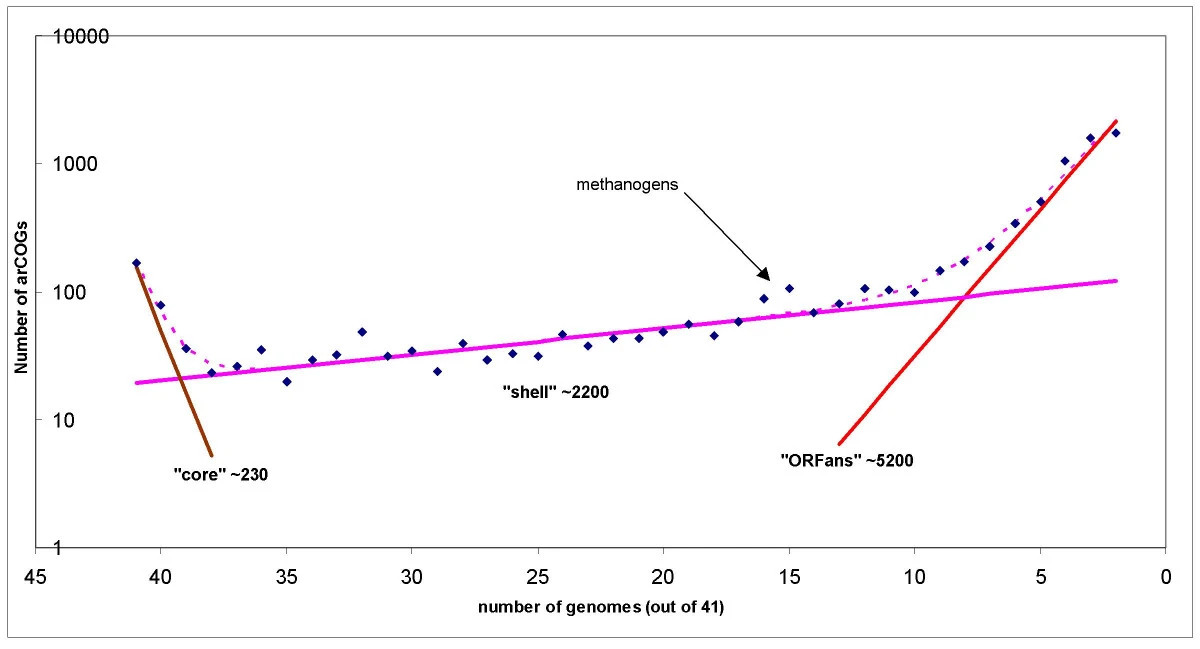
\includegraphics[width=0.48\linewidth]{images/MakarovaPartition.jpg}
%         \label{fig:arCOGs}
%     }
%     \hfill
%     \subfloat[Distribution du nombre d'espèces procaryote dans les eggNOGs]{
%         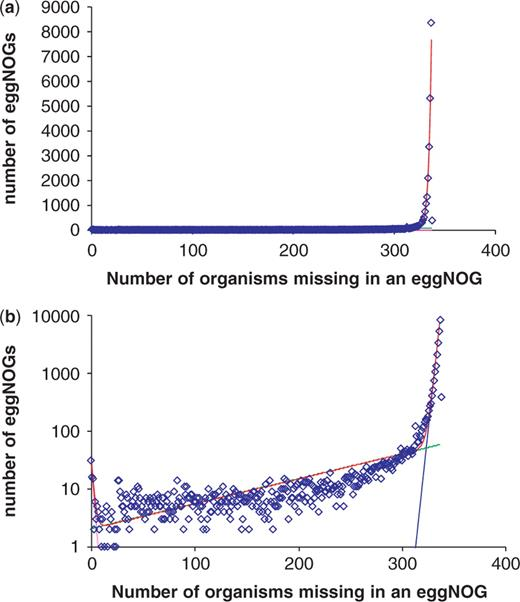
\includegraphics[width=0.48\linewidth]{images/kooninEggNog.jpeg}
%         \label{fig:eggNOGs}
%     }
%     \caption{Distribution du nombre de génomes où une annotation fonctionnelle est retrouvé}
%     \label{fig:parti3}
% \end{figure}

\subsubsection{Représentation des pangénomes de gènes.}

Pour représenter ces pangénomes, il est possible d'utiliser une matrice de présence/absence des gènes (\autoref{fig:panType}B). Cette représentation permet de rapidement identifier le \textit{core genome} ou de trouver les gènes spécifiques à un génome d'intérêt par exemple. Une seconde représentation est celle du diagramme de Venn (\autoref{fig:pangenomeVenn}). À partir du diagramme, on peut rapidement avoir une idée de la proportion de chaque partie, et aussi de la "croissance" du pangénome (cf. \autoref{sec:croissance_pan}). Ces 2 représentations ont l'intérêt d'être simple à calculer et à interpréter, néanmoins, lorsque le nombre de génomes devient trop important, il n'est plus possible de les visualiser correctement. De plus, dans ces représentations, l'information d'organisation des génomes est perdue. 

Une autre approche va représenter les gènes et leur organisation dans une structure de graphe. Dans ce graphe, les familles de gènes constitue les n\oe uds et les relations de voisinages entre les gènes correspondent aux arêtes. Sur la \autoref{fig:graphPanFam}, on peut voir que dans cette représentation, plus des familles ont des gènes voisins, plus le poids de l'arête (épaisseur) augmente. Le graphe de pangénome permet alors d'identifier des structures ou des chemins de familles conservées, ou à l'inverse des régions fortement variables.

\begin{figure}[htbp]
    \centering
    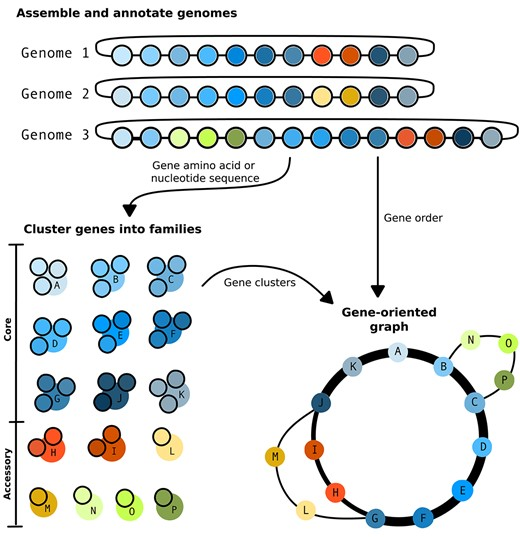
\includegraphics[width=0.8\linewidth]{images/graphePanFam.jpeg}
    \caption[Représentation d'un pangénome de gènes sous forme de graphe]{Représentation d'un pangénome de gènes sous forme de graphe. Extrait de \cite{matthews_gentle_2024}}
    \label{fig:graphPanFam}
\end{figure}

\subsection{Pangénome basé sur les séquences}

\subsubsection{Graphe de pangénome de séquences}
\label{sec:graphSeq}


\subsection{Modélisation de la croissance des pangénomes}
\label{sec:croissance_pan}

Dans l'article original de Tettlin \textit{et al.}, les auteurs s'intéresse à la distribution \textit{core/dispensable} en fonction du nombre de génomes que contient le pangénome. Ils observent que lorsque le nombre de génomes augmente, la part de \textit{core genome} décroît de façon exponentielle. Ce résultat les amène à modéliser la croissance des pangénomes selon une équation exponentielle décroissante. Ce modèle permet alors d'estimer la taille du \textit{core genome} pour un nombre de génome en théorie infinie. Ce modèle permet également de prédire la taille du pangénome, \textit{i.e.}, le nombre de famille de gènes que contient le pangénome avec un nombre infinie de génome. Ils définissent alors 2 types de pangénomes : les pangénomes ouvert et les pangénomes fermés\footnote{ar WELCH et al., 2002 et VAN HAM et al., 200}. Les pangénomes sont considéré comme ouvert lorsque le nombre de gènes ou famille de gènes ajouté au pangénome ne diminue pas avec l'ajout de nouveaux génomes. Le nombre de familles est donc théoriquement infini pour un pangénome ouvert avec une infinité de génome. Les pangénomes fermé quant à eux voit le nombre de nouvelles familles progressivement diminué lors de l'ajout de nouveaux génomes. La courbe de prédiction permet d'identifier un plateau théorique du nombre maximale de familles que contiendra le pangénome avec un nombre de génome infinie. Biologiquement, le pangénome ouvert est attendue pour les espèces sympatrique\footnote{Espèces vivant entouré dans le même environnement que d'autres espèces.} et qui présentent un fort taux de transfert horizontaux, tandis que les espèces vivant dans des niches écologique ou qui ont une faible capacité d'aquisition de gènes extérieurs vont avoir un pangénome fermé.